\documentclass[12pt]{article}

\usepackage{sbc-template}
\usepackage{graphicx,url,setspace,subfig, float}
\usepackage[utf8]{inputenc}
\usepackage[brazil]{babel}

\sloppy

\title{MAC5753 -- Sistemas Operacionais -- 2s2020\\ EP1}

\author{Guilherme Werneck de Oliveira\inst{1}}

\address{Instituto de Matemática e Estatística -- Universidade de São Paulo (USP)\\
  Rua do Matão, 1010 - CEP 05508-090 - São Paulo - SP}

\begin{document}

\maketitle

\begin{abstract}
  This report describes the development and the results obtained from experiments carried out with process schedulers. Two programs were developed, one referring to shell, possh, and the other to the process simulator, ep1. For possh, execl system calls were used to invoke external programs, in addition to the mkdir, kill and link system calls.
  For the process simulator, schedulers were implemented: First-Come First-Served (FCFS), Shortest Remaining Time Next (SRTN) and Round-Robin (RR). The results presented showed that the SRTN performed better than the others, considering the number of processes that reached deadlines and the number of context changes. They also showed that the preemptive scheduling algorithms accounted for the largest number of context changes, with a greater emphasis on RR.
\end{abstract}

\begin{resumo}
  Este relatório descreve o desenvolvimento e os resultados aferidos de experimentos realizados com escalonadores de processos. Foram desenvolvidos dois programas, um referente ao shell, possh, e o outro ao simulador de processos, ep1. Para o possh, foram utilizadas as chamadas de sistema execl para a invocação de programas externos ao desenvolvido, além das chamadas de sistema mkdir, kill e link.
  Já para o simulador de processos, foram implementados os escalonadores: First-Come First-Served (FCFS), Shortest Remaining Time Next (SRTN) e Round-Robin (RR). Os resultados apresentados mostraram que o SRTN teve um desempenho superior aos demais, considerando a quantidade de processos que cumpriram os deadlines e a quantidade de trocas de contexto. Também, mostraram que os algoritmos de escalonamento preemptivos contabilizaram o maior número de trocas de contexto, com um destaque maior para o RR.
\end{resumo}


\section{Introdução}

A democratização da tecnologia tem trazido cada vez mais um grande aumento no desenvolvimento de novos \textit{softwares}. Segundo \cite{clement:20}, foram mais de 2,9 milhões de aplicativos disponibilizados na Google Play Store em junho de 2020.

Com tantas opções, uma das características mais buscadas pelos usuários é a usabilidade. Além disso, um fator de grande importância para a garantia de uma boa usabilidade é a interatividade entre vários aplicativos, ou processos, que competem simultaneamente pelo mesmo \textit{hardware}.

Para que a interatividade seja garantida e que todos os processos seja atendidos, um dos mecanismos necessários em um sistema operacional multiprogramado é o escalonador de processos. Um escalonador de processos é um decisor de qual processo deverá utilizar a CPU naquele instante de acordo com um algoritmo de escalonamento. \cite{tanenbaum:16}.

\section{Descrição do Problema} \label{sec:firstpage}

A tarefa solicitada neste primeiro exercício prático (EP1) da disciplina de Sistemas Operacionais do 2º semestre de 2020 solicita a implementação de um \textit{shell} que possibilita a interação de seu usuário com recursos do sistema operacional e, solicita também, o desenvolvimento de um simulador de processos com três algoritmos de escalonamento inclusos.

O \textit{shell}, chamado de possh, deve conter em seu \textit{prompt} a seguinte estrutura entre chaves: nome do usuário, seguido de @, do diretório atual e finalizado com um espaço em branco após o fechamento das chaves. O \textit{shell} deve permitir a execução dos seguintes binários com seus respectivos argumentos:
\begin{itemize}
	\item /usr/bin/du -hs .
	\item /usr/bin/traceroute www.google.com.br
	\item ./ep1 $<$argumentos do EP1$>$
\end{itemize}

Também deverá incluir as seguintes chamadas de sistema para a interação do usuário:
\begin{itemize}
	\item mkdir $<$diretorio$>$
	\item kill -9 $<$PID$>$
	\item ln -s $<$arquivo$>$ $<$link$>$
\end{itemize}

Além disso, o \textit{shell} também deve suportar a navegação e a edição de comandos implementados pelas bibliotecas GNU \textit{readline} e GNU \textit{history}.

Já o simulador de processos deverá implementar os seguintes escalonadores:
\begin{enumerate}
	\item \textit{First-Come First-Served}
	\item \textit{Shortest Remaining Time Next}
	\item \textit{Round-Robin}
\end{enumerate}

O simulador de processos recebe um arquivo como entrada contendo diversos processos, um em cada linha, no formato nome, t0, dt e \textit{deadline}, onde t0 é o instante de tempo de chegada de um processo no simulador, dt é o tempo de consumo de CPU do processo e \textit{deadline} é o instante de tempo do qual o processo precisa finalizar. Exemplo: processo1 0 5 6.

Uma vez informado através de seus parâmetros de entrada, o simulador deverá gerar um arquivo de saída contendo uma linha para cada processo no formato nome, tf e tr, onde tf é considerado o instante de tempo final do processo e tr é o tempo que o processo levou para executar, ou seja, tf-t0. Também, o arquivo de saída incluí em sua última linha a quantidade de trocas de contexto realizada pelo escalonador selecionado.

\section{Descrição da Solução}

O código-fonte, os arquivos gerados para os testes utilizados pelo simulador de processos e os resultados aferidos estão disponíveis em \url{github.com/werneckg/mestrado/SO/EP1}. Tanto a implementação do \textit{shell} possh quanto a do simulador de processos ep1 foram divididas de acordo com as seguintes estruturas:
\begin{itemize}
	\item possh:
	\begin{itemize}
		\item possh.h, arquivo contendo o cabeçalho das funções utilizadas pelo \textit{shell};
		\item possh.c, implementação das funções utilizadas pelo \textit{shell};
		\item main-possh.c, arquivo contendo a implementação da função principal do \textit{shell}.
	\end{itemize}
	\item ep1:
	\begin{itemize}
		\item ep1.h, arquivo contendo o cabeçalho das funções utilizadas pelo simulador de processos;
		\item ep1.c, implementação das funções utilizadas pelo simulador de processos;
		\item main-ep1.c, arquivo contendo a implementação da função principal do simulador de processos.
	\end{itemize}

\end{itemize}

\subsection{\textit{Shell} possh}

O desenvolvimento do \textit{shell} possh pode ser descrito inicialmente como um laço infinito que recebe entradas, ou comandos, digitadas pelo usuário. Os comandos a serem executados pelo programa foram implementados de duas maneiras. Para os binários \textbf{du}, \textbf{traceroute} e \textbf{ep1}, foram utilizados o \textbf{execl} com os respectivos binários de destino e parâmetros. Já para os comandos \textbf{mkdir}, \textbf{kill} e \textbf{ln} foram utilizadas as próprias chamadas de sistemas consultadas em \cite{kerrisk:20}.

Outra característica importante de citar é a criação de processos filhos, utilizando a chamada de sistema \textbf{fork()}, para não permitir que o processo principal seja encerrado após a execução do \textbf{execl}, uma vez que ele sobre-escreve o processo que o chamou. Essa estratégia é ilustrada na Figura~\ref{fig:fork}.
\begin{figure}[H]
	\centering
	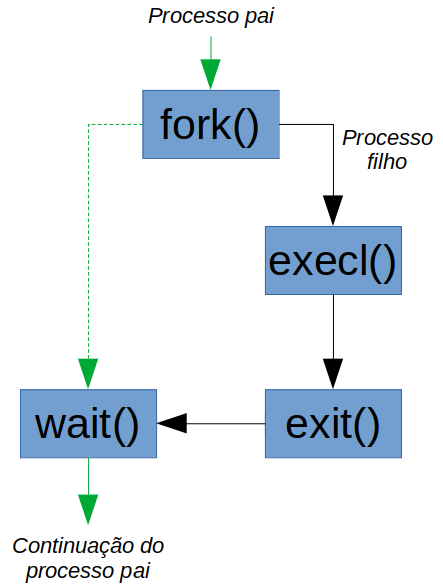
\includegraphics[width=.4\textwidth]{fork.png}
	\caption{Fluxo de execução de processos filhos.}
	\label{fig:fork}
\end{figure}

\subsection{Simulador de Processos ep1}

O simulador de processos implementa os três escalonadores distintos: \textit{First-Come First-Served} (FCFS), \textit{Shortest Remaining Time Next} (SRTN) e o \textit{Round-Robin} (RR) com a possibilidade de parametrização do \textit{quantum}. Além disso, considera que os processos concorram por apenas uma CPU, ou seja, não há processos executados paralelamente.

A quantidade de trocas de contexto contabilizada pelos escalonadores sempre considera a colocação de um processo na CPU, seja pela CPU estar ociosa, por um processo finalizado anteriormente ou pela retirada do processo anterior para a execução do atual candidato.

A decisão de projeto tomada para a implementação desse simulador considera que para os escalonadores FCFS e SRTN o tempo mínimo de permanência de um processo na CPU é de um segundo. Já para o RR o tempo máximo de permanência de um processo na CPU é a quantidade de segundos descrita pelo \textit{quantum} parametrizado.

Todo processo possuí três estados: pronto, executando e finalizado. Também, é simulado por sua respectiva \textit{thread} e é manipulado através de seus semáforos. Como requisitado pela descrição do EP1, cada processo chega no simulador no instante t0. Essa informação é utilizada da seguinte forma: a cada instante de tempo, aqui considerado um segundo, o simulador checa se existe algum processo no instante t. Se existe, ele avalia de acordo com o algoritmo em execução, se o processo deve ou não ser colocado na CPU. Se não há processo no instante t, ele avalia se o processo em execução deve se manter na CPU. Caso o processo em execução tenha finalizado seu uso da CPU, o simulador apenas incrementa o tempo t.

Toda a gestão de execução dos processos é realizada pelo escalonador. É ele que decide quando, qual e por quanto tempo um processo vai utilizar a CPU. Por exemplo, quando um processo, chamado de candidato, chega no simulador ele é avaliado de acordo com seu estado para que, dessa forma, o escalonador tome uma decisão. Se seu estado for "pronto" e não existir processos utilizando a CPU, o escalonador iniciar a \textit{thread} do processo e, consequentemente, seu semáforo. Se seu estado for "pronto" e existir um processo utilizando a CPU, o escalonador fará a decisão baseada no algoritmo escolhido. Se essa decisão for por trocar o processo atual que está utilizado a CPU pelo processo candidato naquele instante t, o escalonador para a execução do processo atual por meio de seu semáforo e inicia a execução do processo candidato. Também é possível que o processo candidato já esteja como estado "executando", nesse caso o escalonador para o processo atual e libera o semáforo do processo candidato para seu uso da CPU.

Após essa avaliação e decisão, o escalonador aguarda a execução do processo e decrementa seu dt de acordo com a quantidade de segundos consumidos pelo processo. Se seu dt for 0, significa que o processo finalizou sua execução. Com isso, a \textit{thread} do processo é finalizada e processo passa a ter o estado de "finalizado".

Por fim, sempre que um processo é finalizado a contabilidade de seu tf e tr é realizada e armazenada no arquivo de saída parametrizado no início da execução do simulador.

\section{Resultados Obtidos}

Os resultados apresentados foram obtidos a partir da execução do simulador de processos em duas máquinas distintas:
\begin{itemize}
	\item \textbf{Máquina A (física)}: Processador Intel® Core i5 com 4 CPUs, 6 GB de memória RAM e sistema operacional Ubuntu 20.04.1 LTS;
	\item \textbf{Máquina B (virtual na nuvem Microsoft® Azure)}: Processador Intel® Xeon com 2 vCPUs, 8 GB de memória RAM e sistema operacional Debian 10.5.
\end{itemize}

Foram gerados 30 arquivos de entrada para cada tipo de instância separadas por: pequenas instâncias (S) com 20 processos, médias instâncias (M) com 50 processos e grandes instâncias (L) com 100 processos. Os arquivos gerados consideraram o tempo de processamento dos processos entre 1 e 10 segundos. Consequentemente, o tempo de processamento médio dos processos para cada arquivo gerado foi de 5 segundos.

Os valores apresentados nos gráficos foram obtidos a partir da execução do simulador de processos para cada uma das 30 entradas por tipo de instância aferidos com um intervalo de 95\% de confiança.

Para a definição do \textit{quantum} do escalonador RR, foram realizados alguns testes iniciais o considerando abaixo da média, na média e acima da média do tempo de processamento dos processos. Foi notado que quando parametrizado abaixo da média, havia uma grande quantidade de processos que perdiam seus \textit{deadlines} para todas as instâncias S, M e L. Já quando considerado acima da média do tempo de processamento, a quantidade de processos que perdiam o \textit{deadline} reduzia. No entanto, para manter um intervalo em que não houvesse grande perda de \textit{deadlines} e para que os processos não monopolizassem o uso da CPU, o \textit{quantum} escolhido foi de 7 segundos.


\subsection{Cumprimento de Deadline}

Considere os gráficos da cor azul os resultados obtidos da execução do simulador de processos na máquina A e os gráficos da cor verde na máquina B. Uma característica importante observada foi que, apesar do simulador ter sido executado em máquinas com diferentes quantidades de CPU, o comportamento e os resultados calculados pelo simulador foram iguais. Esse era um resultado esperado uma vez em que o simulador considera apenas o uso de uma CPU por vez. Outro fato observado foi na velocidade de execução do código. Foi percebido uma leve diferença no tempo de execução em ambas. Apesar de ser pouca a diferença, foi notável.

Os gráficos ilustrados na Figura~\ref{fig:cdS} mostram que o SRTN teve o melhor desempenho entre os escalonadores, mas não muito distante do FCFS. Outro fator observado foi que o RR teve o pior desempenho entre os escalonadores com a maior taxa de erro calculada.

\begin{figure}[H]
	\centering
	\subfloat[Máquina A. \label{fig:cdS_A}]{
		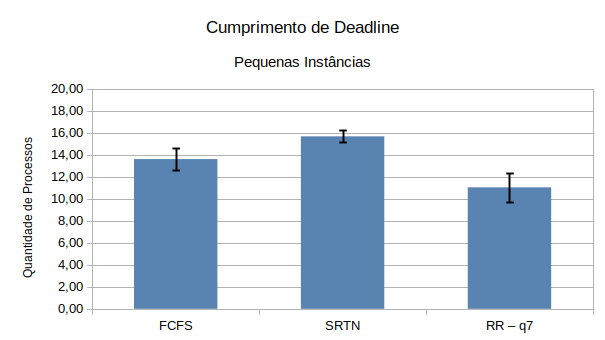
\includegraphics[width=0.48\textwidth]{cdS_A.png}
	}\hfill
	\subfloat[Máquina B. \label{fig:cdS_B}]{
		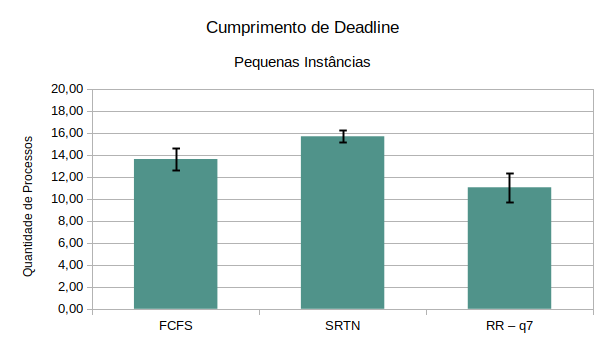
\includegraphics[width=0.48\textwidth]{cdS_B.png}
	}
	\caption{Cumprimento de deadline para pequenas instâncias.}
	\label{fig:cdS}
\end{figure}

\begin{figure}
	\centering
	\subfloat[Máquina A. \label{fig:cdM_A}]{
		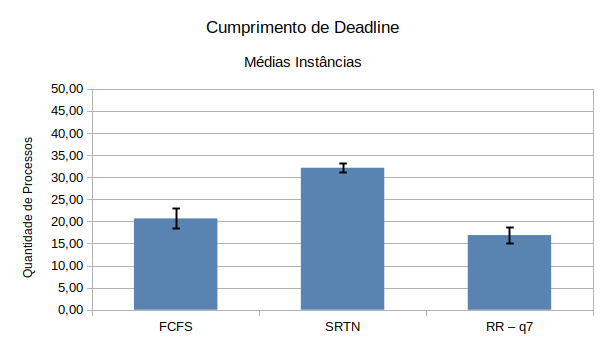
\includegraphics[width=0.48\textwidth]{cdM_A.png}
	}\hfill
	\subfloat[Máquina B. \label{fig:cdM_B}]{
		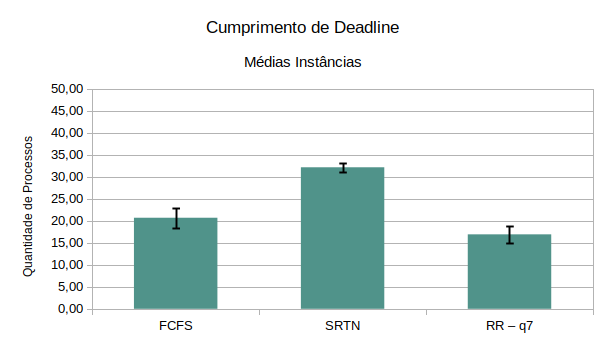
\includegraphics[width=0.48\textwidth]{cdM_B.png}
	}
	\caption{Cumprimento de deadline para médias instâncias.}
	\label{fig:cdM}
\end{figure}

\begin{figure}
	\centering
	\subfloat[Máquina A. \label{fig:cdL_A}]{
		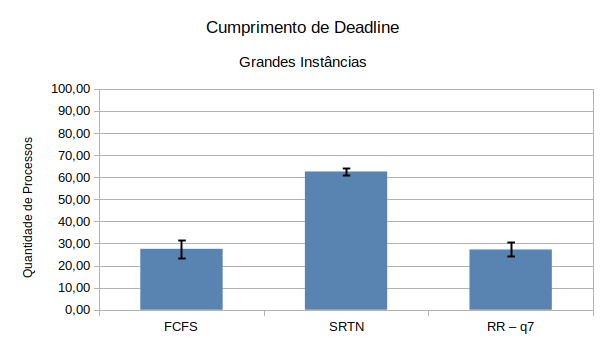
\includegraphics[width=0.48\textwidth]{cdL_A.png}
	}\hfill
	\subfloat[Máquina B. \label{fig:cdL_B}]{
		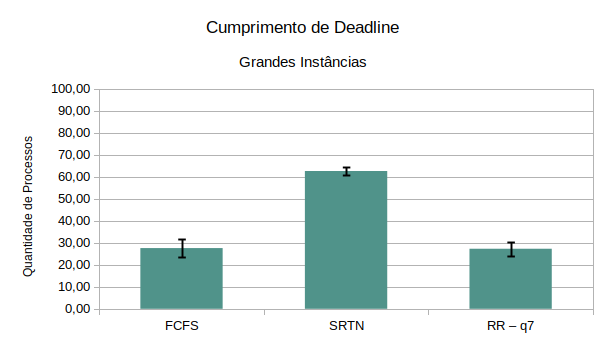
\includegraphics[width=0.48\textwidth]{cdL_B.png}
	}
	\caption{Cumprimento de deadline para grandes instâncias.}
	\label{fig:cdL}
\end{figure}

A Figura~\ref{fig:cdM} ilustra a mesma tendência de resultados em que o SRTN teve o melhor desempenho entre os escalonadores. Porém, os resultados mostram uma porcentagem maior de processos que perderam o \textit{deadline}.

Já a Figura~\ref{fig:cdL} corrobora com o fato de que quanto maior a quantidade de processos a concorrer por um único recurso, maior deverá ser o \textit{deadline} dos processos. Outra característica observada foi que o desempenho do RR ficou muito próximo ao desempenho do FCFS, isso se deve ao fato da parametrização do \textit{quantum} ter sido acima da média do tempo de processamento dos processos.

\subsection{Trocas de Contexto}

Como citado anteriormente, a quantidade de trocas de contexto contabilizada pelos escalonadores sempre considera a colocação de um processo na CPU, seja pela CPU estar ociosa, por um processo finalizado anteriormente ou pela retirada do processo anterior para a execução do atual candidato.

\begin{figure}
	\centering
	\subfloat[Máquina A. \label{fig:tcS_A}]{
		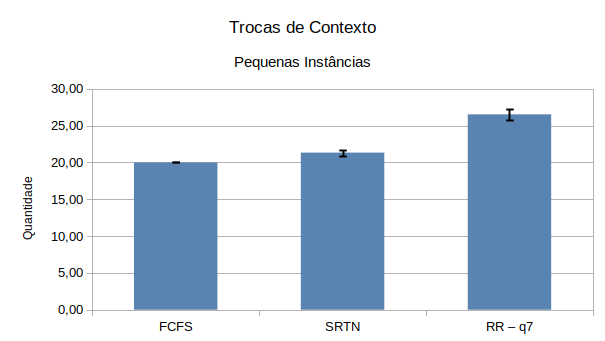
\includegraphics[width=0.48\textwidth]{tcS_A.png}
	}\hfill
	\subfloat[Máquina B. \label{fig:tcS_B}]{
		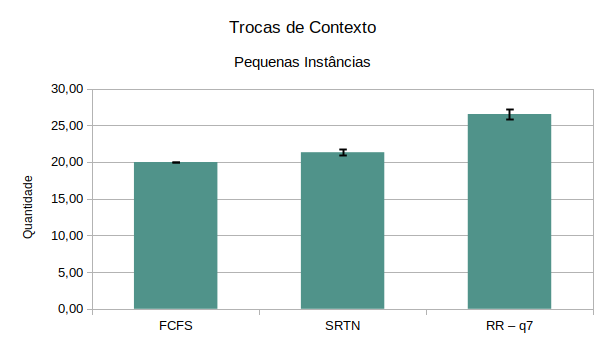
\includegraphics[width=0.48\textwidth]{tcS_B.png}
	}
	\caption{Trocas de contexto para pequenas instâncias.}
	\label{fig:tcS}
\end{figure}

A Figura~\ref{fig:tcS} mostra uma quantidade crescente de trocas de contexto entre o escalonadores FCFS, SRTN e RR, respectivamente. São resultados esperados, uma vez em que os algoritmos SRTN e RR realizam preempção.

\begin{figure}
	\centering
	\subfloat[Máquina A. \label{fig:tcM_A}]{
		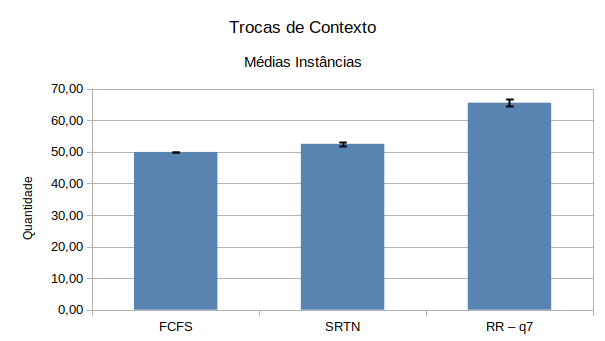
\includegraphics[width=0.48\textwidth]{tcM_A.png}
	}\hfill
	\subfloat[Máquina B. \label{fig:tcM_B}]{
		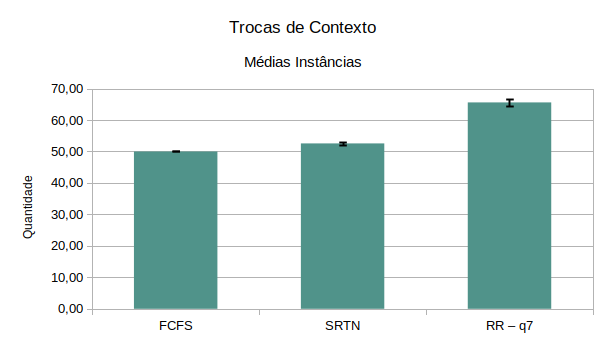
\includegraphics[width=0.48\textwidth]{tcM_B.png}
	}
	\caption{Trocas de contexto para médias instâncias.}
	\label{fig:tcM}
\end{figure}

\begin{figure}
	\centering
	\subfloat[Máquina A. \label{fig:tcL_A}]{
		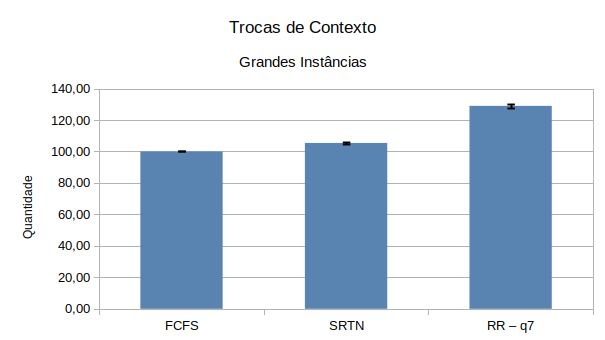
\includegraphics[width=0.48\textwidth]{tcL_A.png}
	}\hfill
	\subfloat[Máquina B. \label{fig:tcL_B}]{
		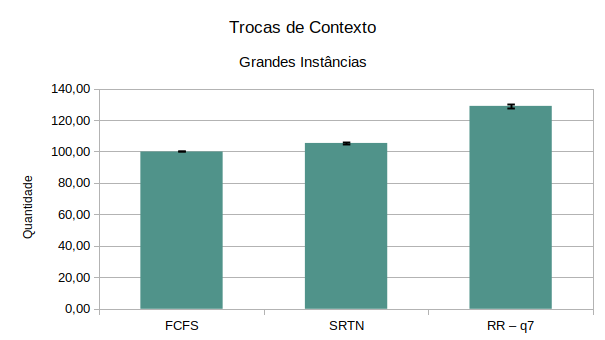
\includegraphics[width=0.48\textwidth]{tcL_B.png}
	}
	\caption{Trocas de contexto para grandes instâncias.}
	\label{fig:tcL}
\end{figure}

Uma característica observada na Figura~\ref{fig:tcS}, Figura~\ref{fig:tcM} e Figura~\ref{fig:tcL} é que a quantidade de trocas de contexto realizadas pelo SRTN foi muito próxima a quantidade de trocas de contexto realizadas pelo FCFS. Apesar disso, os resultados demonstram que o SRTN teve o melhor desempenho nos testes, tanto no cumprimento dos \textit{deadlines} quanto na quantidade de trocas de contexto.

\clearpage

\bibliographystyle{sbc}
\bibliography{sbc-template}

\end{document}
